
%====================================== COMPUTER VISION ========================= 

% Slide 1: Tổng quan + Pipeline
\begin{frame}{Tổng quan CV}
\begin{block}{Định nghĩa \& Mục tiêu}
CV cho máy tính \textbf{hiểu và phân tích hình ảnh/video} → phân loại, phát hiện, theo dõi, ước lượng tư thế.  
Mục tiêu: \textbf{Nhanh, chính xác, quy mô lớn}.
\end{block}
\begin{figure}
    \centering
    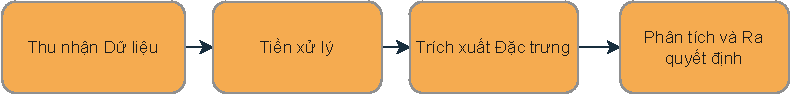
\includegraphics[width=0.8\textwidth]{vision_flow-crop.pdf}
    \caption{Pipeline CV: Thu nhận → Tiền xử lý → Trích xuất đặc trưng → Ra quyết định.}
\end{figure}
\end{frame}

% Slide 2: Bài toán CV cốt lõi
\begin{frame}{Bài toán CV cốt lõi}
\begin{itemize}
    \item Phân loại ảnh
    \item Phát hiện đối tượng (bounding box)
    \item Phân đoạn ảnh: ngữ nghĩa / thể hiện
    \item Ước lượng Tư thế Người (HPE) → keypoints
\end{itemize}
\end{frame}

% Slide 3: CNN + ViT
\begin{frame}{CNN \& Vision Transformer}
\begin{columns}[T]
\begin{column}{0.5\textwidth}
\textbf{CNN}: Tích chập + Pooling → học đặc trưng phân cấp
\begin{figure}
\centering
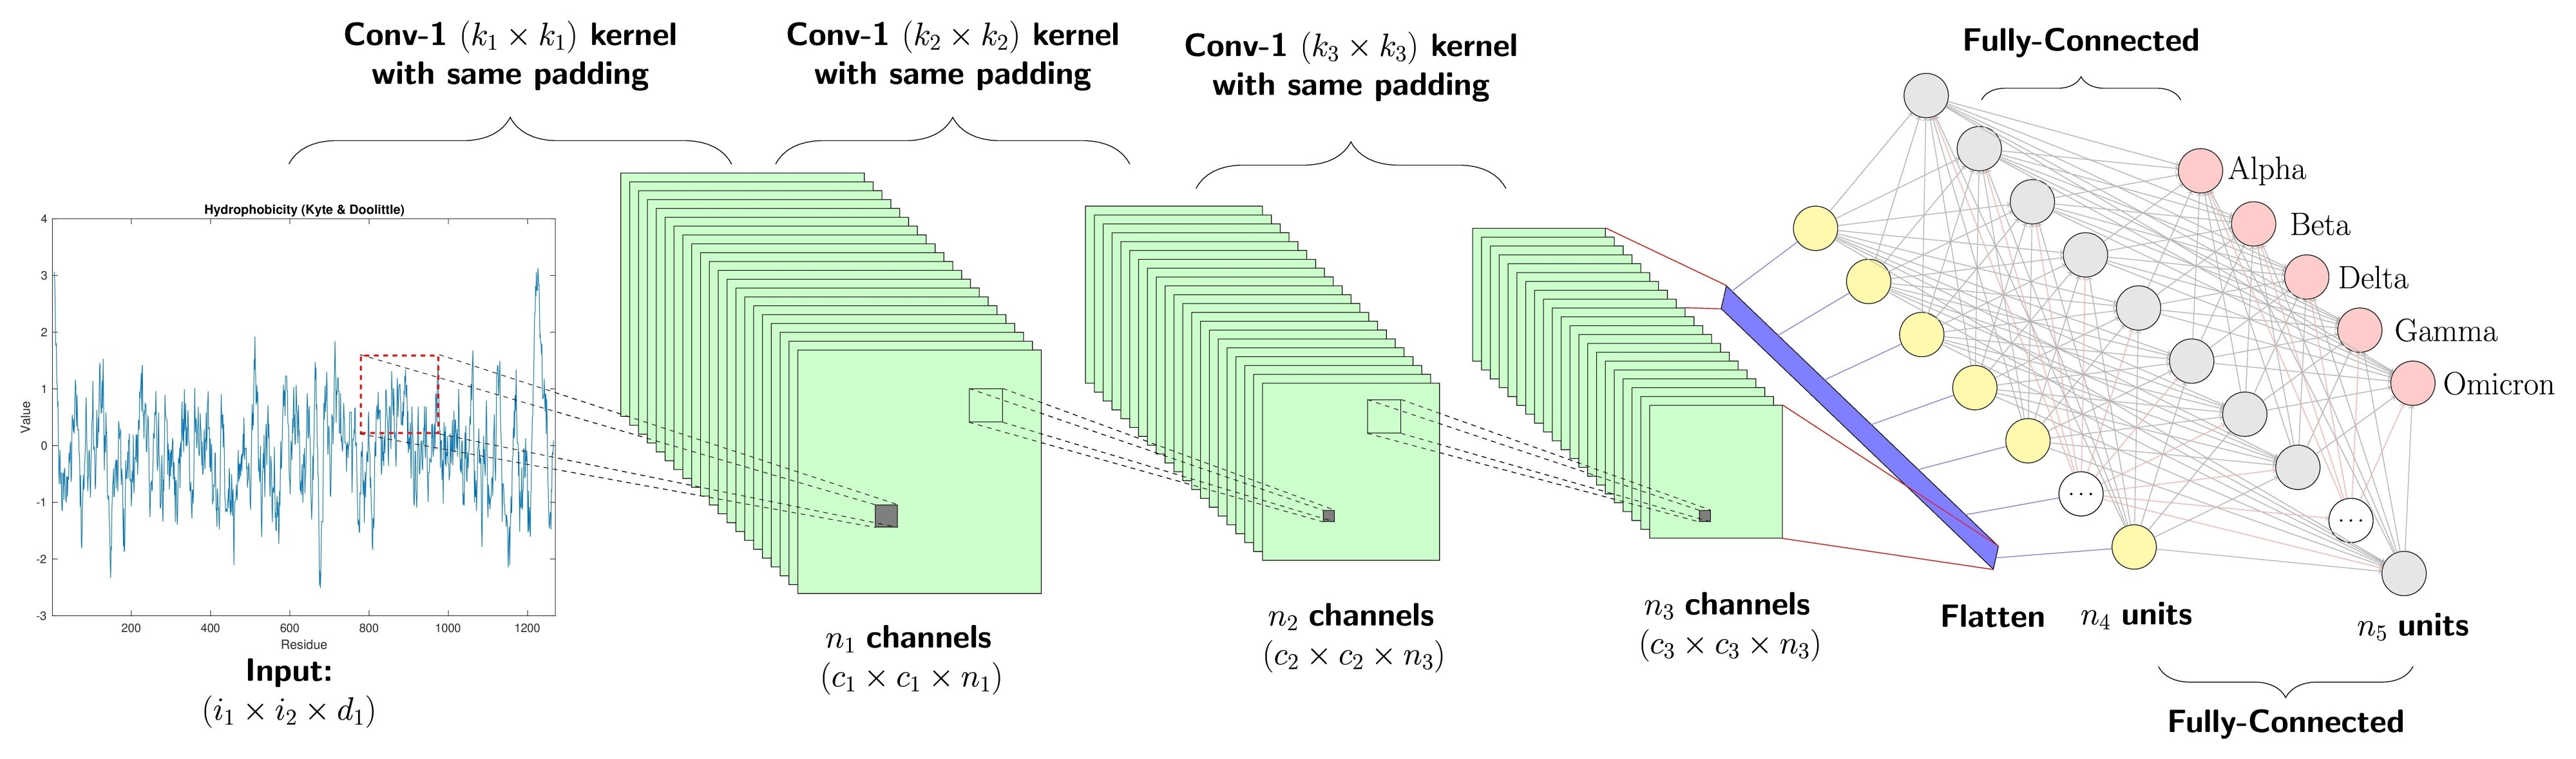
\includegraphics[width=0.9\textwidth]{2_2_convolution.jpeg}
\caption{CNN Operations}
\end{figure}
\end{column}
\begin{column}{0.5\textwidth}
\textbf{ViT}: Chia ảnh thành patches → Self-Attention → quan hệ toàn cục
\begin{figure}
\centering
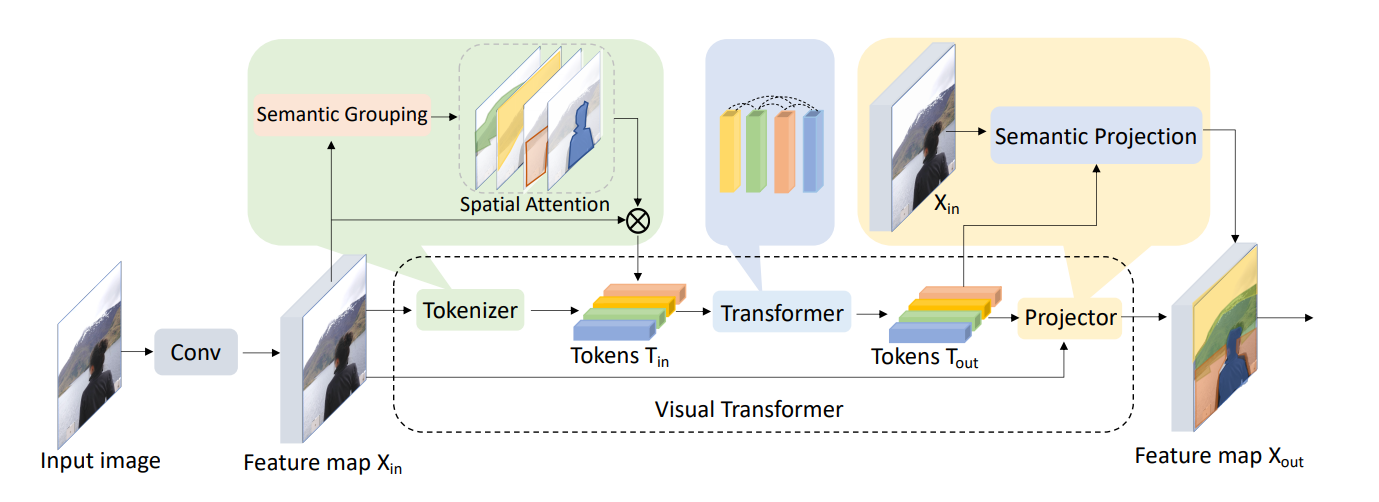
\includegraphics[width=0.9\textwidth]{visual_transformer.png}
\caption{Vision Transformer}
\end{figure}
\end{column}
\end{columns}
\end{frame}

% Slide 4: Datasets & Metrics - Detailed

\begin{frame}{Tập dữ liệu \& Metrics trong CV}
\begin{columns}[T]

% Column 1: Datasets
\begin{column}{0.55\textwidth}
\begin{block}{Tập dữ liệu chính}
\begin{itemize}
    \item \textbf{ImageNet} \cite{deng2009imagenet}: >14 triệu ảnh, ~20,000 nhãn. Chuẩn cho \textbf{phân loại ảnh}.
    \item \textbf{COCO} \cite{lin2014microsoft}: Hơn 330k ảnh, có \textbf{bounding box}, \textbf{segmentation}, \textbf{keypoints}. Chuẩn cho phát hiện đối tượng & phân đoạn.
    \item \textbf{MPII Human Pose}: ~25k ảnh, 16 keypoints trên cơ thể người. Chuẩn cho HPE.
    \item \textbf{COCO Keypoints}: Mở rộng COCO cho 17 keypoints, hỗ trợ HPE thời gian thực.
\end{itemize}
\end{block}
\end{column}

% Column 2: Metrics
\begin{column}{0.45\textwidth}
\begin{block}{Metrics}
\begin{itemize}
    \item IoU – Trùng khớp hộp giới hạn
    \item mAP – Hiệu suất phát hiện đối tượng
    \item F1-score – Trung bình điều hòa Precision & Recall
    \item OKS – Độ chính xác keypoints HPE
\end{itemize}
\end{block}
\end{column}

\end{columns}
\end{frame}
